\documentclass[dvipdfmx]{beamer}
\usepackage{mytheme}
\setbeamercovered{transparent=0}

\usepackage{listings, jlisting}
\lstset{%
 language={python},
 morekeywords={end, function},
 backgroundcolor={\color[gray]{.9}},%
 basicstyle={\small\ttfamily},%
 identifierstyle={\small\ttfamily},%
 commentstyle={\small\ttfamily\color[gray]{.25}},%
 keywordstyle={\bfseries},%
 ndkeywordstyle={\small\ttfamily},%
 stringstyle={\small\ttfamily},
 frame={tb},
 breaklines=true,
 %columns=[l]{fullflexible},%
 numbers=left,%
 xrightmargin=0zw,%
 xleftmargin=3zw,%
 numberstyle={\scriptsize},%
 stepnumber=1,
 numbersep=1zw,%
 lineskip=-0.5ex%
}


\newcommand{\textblue}[1]{\textcolor{blue}{#1}}

\title{まっくろわーるど}
\subtitle{じゅりあらんぐッ!}
\author{yomichi}
\date{JuliaTokyo \#3 2015/04/25}

\begin{document}

\begin{frame}
  \titlepage
  スライドとサンプルコード \\ 
  https://github.com/yomichi/JuliaTokyo3
\end{frame}

\begin{frame}[containsverbatim]
  \frametitle{自己紹介}
  \begin{columns}
    \begin{column}{.8\linewidth}
  \begin{itemize}
    \item HN : 夜道, yomichi
    \item twitter : \verb|@yomichi_137|
    \item ぽすどくにねんせい
      \begin{itemize}
        \item 統計物理学・計算物理学
        \begin{itemize}
          \item 主にモンテカルロ法とか
          \item 言語はC++, Python, \textblue{Julia}
        \end{itemize}
      \end{itemize}
    \item イベント(勉強会)実況勢
      \begin{itemize}
        \item 最近だと全ゲ連(同人ゲーム開発)とか、PyConJP (Python) とか、\textblue{JuliaTokyo}とか
      \end{itemize}
    \item Julia nightly build 勢
    \item Julia の開発環境は REPL と Vim
    \item コミケでJulia 本出したりしてます
      \begin{itemize}
        \item blog とか締め切りがないので書けません><
        \item 抽選受かっていたら次の夏にも出します
          \begin{itemize}
            \item 多分今回の話をもう少し詳しく書きます
          \end{itemize}
      \end{itemize}
  \end{itemize}
\end{column}
\begin{column}{.3\linewidth}
  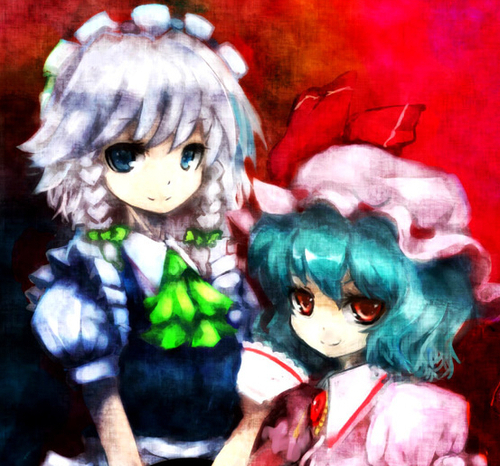
\includegraphics[width=\linewidth]{sakuremi.jpg}

  (thanks \verb|@am_11|)
\end{column}
  \end{columns}
\end{frame}

\begin{frame}
  \frametitle{今日のお話}
  \tableofcontents
  \begin{itemize}
    \item メタプログラミングとかマクロ展開とかのお話です
      \begin{itemize}
        \item (Julia の中では)難しそう or 難しいためか余り触れられてこない話
        \item 確実に30分では終わらないので適当に飛ばします
          \begin{itemize}
            \item 一応スライドだけでも読めるつもりで作ったので、興味ある方はあとでゆっくりとどうぞ
            \item いつものことですが公式ドキュメントが一番詳しくてわかりやすく、ほぼ常に最新なので、英語が苦じゃない人はそちらがおすすめ
          \end{itemize}
      \end{itemize}
    \item 未確認で進行形ネタを仕込もうかと思ったけれどそんな余裕がありませんでした
      \begin{itemize}
        \item なのでタイトルは出オチです
      \end{itemize}
  \end{itemize}
\end{frame}
\section{\texttt{Symbol} 型と\texttt{Expr} 型 -- Julia の抽象構文木}
\begin{frame}
  \frametitle{Outline}
  \tableofcontents[currentsection]
\end{frame}

\begin{frame}[containsverbatim]
\frametitle{Julia の抽象構文木(AST)}
\begin{columns}
\begin{column}{.65\linewidth}
  \begin{itemize}
    \item 例えば\verb|x + (y + z)| という式はJulia の中の人からは右図のように木構造(抽象構文木)として見えている
      \begin{itemize}
        \item \verb|:call| は関数呼び出しの意味
        \item \verb|+| は中置が認められているというだけで普通の関数であることに注意
        \item つまり正確には \verb| +(x, +(y, z))|
      \end{itemize}
  \item Julia は式をこのように抽象構文木に変換して、それから式の評価をしている
    \begin{itemize}
      \item この構造をそのまま保持することで、式やプログラムそのものをデータとして扱える(=\textblue{同図像性})
      \item プログラムを生成するプログラムも書ける(=\textblue{メタプログラミング})
    \end{itemize}
  \end{itemize}
\end{column}
\begin{column}{.55\linewidth}
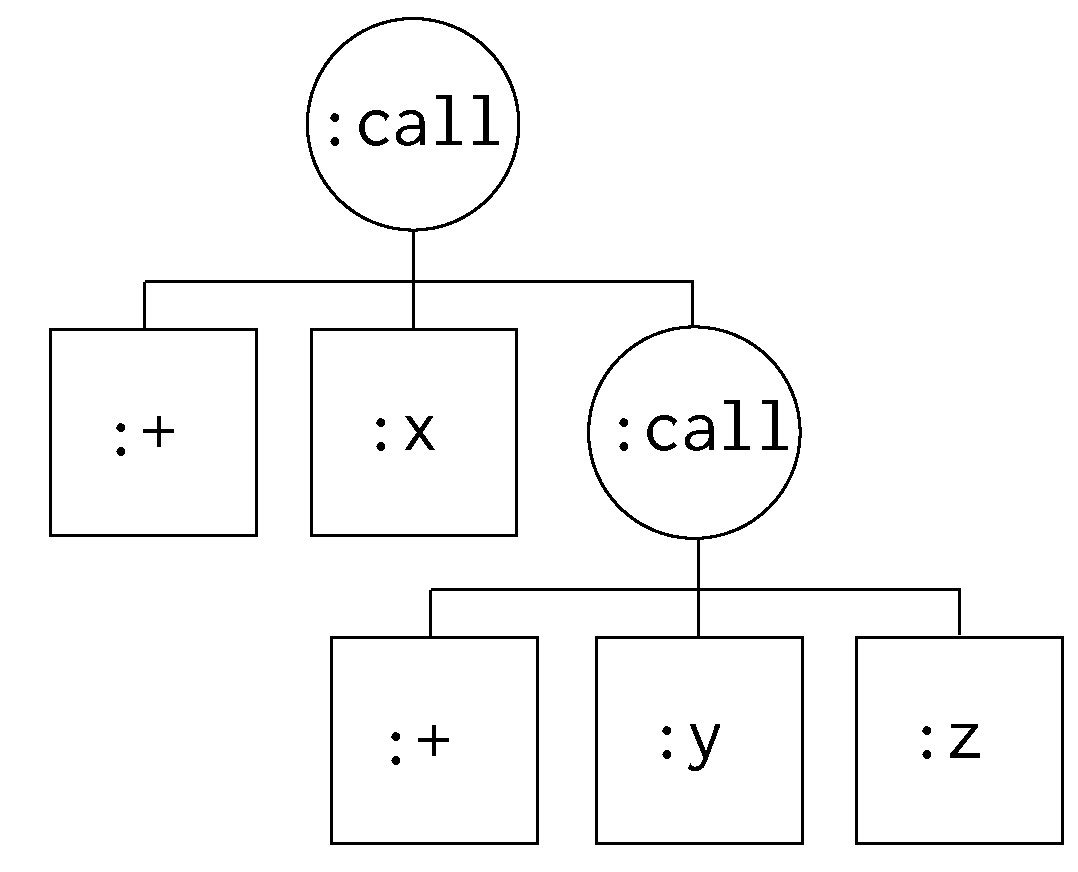
\includegraphics[width=.8\linewidth]{ast.pdf}
\end{column}
\end{columns}
\end{frame}

\begin{frame}[containsverbatim]
\frametitle{Julia の抽象構文木(AST) と\texttt{Symbol}型、 \texttt{Expr}型}
\begin{itemize}
  \item Julia における最も重要な型(データ構造)のうち2つが\verb|Symbol| と\verb|Expr| である
    \begin{itemize}
      \item \verb|Symbol| は識別子・変数名を表す型
      \item \verb|Expr| はJulia そのものの抽象構文木(AST)を表す型
    \end{itemize}
  \item これらの型のオブジェクト(シンボル、AST)は\verb|:()|や\verb|quote ... end| を用いることで作ることができる
\end{itemize}
\begin{lstlisting}
julia> s = :x
:x

julia> typeof(s)
Symbol

julia> ex = :(x + 1)
:(x + 1)

julia> typeof(ex)
Expr
\end{lstlisting}
\end{frame}

\begin{frame}[containsverbatim]
\frametitle{Julia の抽象構文木(AST) と\texttt{Symbol}型、 \texttt{Expr}型}
\begin{itemize}
  \item \verb|Expr| は\verb|head, args, typ| の3つのfield を持つ
    \begin{enumerate}
      \item \verb|head| は行う操作
      \item \verb|args| は操作の対象(引数)
      \item \verb|typ| は結果の型(確定していれば)
        \begin{itemize}
          \item ほとんどの場合で\verb|Any| であり、気にする必要はほとんど無い
        \end{itemize}
    \end{enumerate}
  \item \verb|Base.dump| でまとめて表示できる
    \item \verb|Base.Meta.show_sexpr| を使うとS式で表示できる
\end{itemize}
\begin{lstlisting}
julia> dump(ex)
Expr
  head: Symbol call
  args: Array(Any,(3,))
    1: Symbol +
    2: Symbol x
    3: Int64 1
  typ: Any

julia> Base.Meta.show_sexpr(ex)
(:call, :+, :x, 1)
\end{lstlisting}
\end{frame}

\begin{frame}[containsverbatim]
\frametitle{Julia の抽象構文木(AST) と\texttt{Symbol}型、 \texttt{Expr}型}
\begin{itemize}
  \item AST は木構造なので節と葉を持つ
    \begin{itemize}
      \item 節は\verb|Expr| 型
      \item 葉は\verb|Symbol| 型の値(変数名)かリテラル(数値型・文字列型)
      \item 今回、簡単のため\verb|Expr|, \verb|Symbol|, リテラルをすべてまとめてAST と呼ぶ
    \end{itemize}
\end{itemize}
\begin{lstlisting}
julia> dump( :( x + ( y + z ) ) )
Expr
  head: Symbol call
  args: Array(Any,(3,))
    1: Symbol +
    2: Symbol x
    3: Expr
      head: Symbol call
      args: Array(Any,(3,))
        1: Symbol +
        2: Symbol y
        3: Symbol z
      typ: Any
  typ: Any
\end{lstlisting}
\end{frame}

\begin{frame}[containsverbatim]
\frametitle{変数補間(interpolation)}
\begin{itemize}
  \item quote でAST を作るときに、\verb|$| を使うことで変数や式の値を入れることができる
    \begin{itemize}
      \item 文字列(\verb|" "|)やプロセス(\verb|` `|)における補間と同じ
    \end{itemize}
\end{itemize}
\begin{lstlisting}
julia> y = 42
42

julia> :(x = y)
:(x = y)

julia> :(x = $y)
:(x = 42)

julia> :(x = sin(1.0))
:(x = sin(1.0))

julia> :(x = $(sin(1.0)))
:(x = 0.8414709848078965)
\end{lstlisting}
\end{frame}

\begin{frame}[containsverbatim]
\frametitle{変数補間で\texttt{Symbol} を陽に残す}
\begin{itemize}
  \item 例えば\verb|Symbol| を受け取る関数を呼び出す式をquote したいときに、その\verb|Symbol| を変数補間で与えたい
  \item この時そのまま\verb|$s| と書くと、\verb|Symbol| ではなく名前が書き込まれてしまう
    \begin{itemize}
      \item ほとんどのマクロではこの挙動の方が都合がいい
    \end{itemize}
  \item 配列かタプルに隠して埋め込み、後から取り出せばよい
\end{itemize}

\begin{lstlisting}
julia> :( foo(:a) ) # これが欲しい
:(foo(:a))

julia> s = :a ;
julia> :( foo($s) ) # 直接埋め込むとダメ
:(foo(a))

julia> :( foo( $[s]...) ) # 一度配列に隠す
:(foo([:a]...))

julia> :( foo( $(s,)...) ) # タプルでも良い
:(foo((:a,)...))
\end{lstlisting}

\end{frame}

\begin{frame}[containsverbatim]
\frametitle{式の評価}
\begin{itemize}
  \item \verb|eval| 関数にAST を渡すことで、AST の評価を行える
  \item AST に未定義な変数を含めることができるが、定義する前にAST を評価するともちろんエラーが出る
\end{itemize}
\begin{lstlisting}
julia> x
ERROR: UndefVarError: x not defined

julia> ex = :(2 * x)
:(2x)

julia> eval(ex)
ERROR: UndefVarError: x not defined

julia> x = 42
42

julia> eval(ex)
84
\end{lstlisting}
\end{frame}

\begin{frame}[containsverbatim]
\frametitle{式の操作}
\begin{itemize}
  \item \verb|Expr| は\verb|immutable| ではないので、AST を操作することができる
\end{itemize}
\begin{lstlisting}
julia> ex
:(2x)

julia> x, eval(ex)
(42,84)

julia> ex.args[2] = 20;

julia> ex
:(20x)

julia> x, eval(ex)
(42,840)
\end{lstlisting}
\end{frame}

\begin{frame}[containsverbatim]
\frametitle{第一級オブジェクトとしてのAST \\ -- 同図像性(Homoiconic)}
\begin{itemize}
  \item ソースコードをquote することでAST を生み出すことができた
    \begin{itemize}
      \item \verb|Expr| のコンストラクタを呼び出して作ることもできる
      \item \verb|parse| 関数を使うことで、文字列から作ることもできる
    \end{itemize}
\end{itemize}
\begin{lstlisting}
julia> parse("x+1")
:(x + 1)
\end{lstlisting}
\begin{itemize}
  \item もちろん関数に渡したり関数から受け取ったりできる
  \begin{itemize}
    \item 既に\verb|eval| や\verb|dump|、\verb|parse| といった実例を見てきた
    \item AST を渡すと別のAST に変換する関数を作ることもできる
  \end{itemize}
  \item \verb|eval| に渡すことでいつでもAST を評価・実行できる
  \item このように、自分自身のAST そのものをデータとして扱える言語の性質をhomoiconic と呼ぶ
    \begin{itemize}
      \item AST(プログラム)を自動生成するプログラムを簡単に書ける -- メタプログラミング
      \item マクロを使うことで、より自然な構文の書き換えを行うことができる
    \end{itemize}
\end{itemize}
\end{frame}


\section{マクロシステム}
\begin{frame}
  \frametitle{Outline}
  \tableofcontents[currentsection]
\end{frame}

\begin{frame}[containsverbatim]
\frametitle{マクロ}
\begin{itemize}
  \item マクロは\verb|macro| キーワードで定義して、\verb|@name| という形で呼び出す
  \item マクロがやること
    \begin{enumerate}
      \item 引数をそれぞれ\verb|:()| でquote して
      \item 普通の関数と同様に何か仕事して
      \item 返ってきた値を\verb|eval| する
    \end{enumerate}
  \item AST を受け取ってAST を返す関数の場合、いちいち\verb|quote| や\verb|eval| をする必要があった
    \begin{itemize}
      \item \verb|eval( foo( :( x+1 ) ) ) |
    \end{itemize}
  \item マクロでは \verb|@foo(x+1)| と書ける
    \begin{itemize}
      \item \verb|@foo x+1| のようにも書ける
    \end{itemize}
  \item マクロは関数と違って健全であるという特徴もある
    \begin{itemize}
      \item 説明は次頁
    \end{itemize}
\end{itemize}
\end{frame}

\begin{frame}[containsverbatim]
\frametitle{変数捕捉と健全な(hygienic)マクロ}
\begin{itemize}
  \item マクロはASTを変換(マクロ展開)して、新しいASTを呼び出し元に貼り付ける
    \item 展開されたASTに含まれる名前が、呼び出し元の文脈にあるものと衝突する事がある(=変数捕捉)
    \begin{enumerate}
      \item 必要な名前が呼び出し元で別の値に束縛されている事がある
      \item 呼び出し元の変数を再束縛してしまう
    \end{enumerate}
  \item 名前の付け方に細工をすることで回避する
    \begin{enumerate}
    \item マクロが定義されているモジュール名を使って名前を修飾する
    \item 変数に値を代入するときは、重複しない(今まで作られていなくて、これからも作られない)名前を生成して変数名とする
      \begin{itemize}
        \item \verb|Base.gensym| で生成可能
      \end{itemize}
    \end{enumerate}
    \item \textcolor{blue}{Julia のマクロ展開では全て自動でやってくれる(健全なマクロ)}
\end{itemize}
\end{frame}

\begin{frame}[containsverbatim]
  \frametitle{変数捕捉と健全なマクロ}
\begin{itemize}
  \item \textblue{\texttt{Base.macroexpand}} を使うとマクロ展開した結果を得ることができる
    \begin{itemize}
      \item 関数なのでquote が必要
    \end{itemize}
\end{itemize}
\begin{lstlisting}
module JT3 # 以下全てのマクロはこのモジュール内にある
macro setx_A()
  :( x = sin(1.0) )
end
end
\end{lstlisting}

\begin{lstlisting}
julia> macroexpand( :( JT3.@setx_A ) )
:(#30#x = JT3.sin(1.0))
\end{lstlisting}

\begin{enumerate}
  \item \verb|sin| を\verb|JT3| で修飾することで、呼び出し元が\verb|sin| を隠蔽しているかどうかを気にしなくてよくなる
    \begin{itemize}
      \item \verb|JT3.sin| は(名前の隠蔽をしていなければ)\verb|Base.sin| になる
    \end{itemize}
  \item \verb|#30#x| という名前を作ることで、呼び出し元に\verb|x| があるかどうかを気にしなくてよくなる
\end{enumerate}

\end{frame}

\begin{frame}[containsverbatim]
\frametitle{変数捕捉と健全なマクロ}
\begin{lstlisting}
macro setx_A()
   :( x = sin(1.0) )
end
\end{lstlisting}
\begin{itemize}
  \item Julia が自動的に\verb|x| を保護してくれるために、残念ながらこのマクロを使っても呼び出し元の\verb|x| に変化はおきない
\end{itemize}
\begin{lstlisting}
julia> x
ERROR: UndefVarError: x not defined

julia> JT3.@setx_A
0.8414709848078965

julia> x
ERROR: UndefVarError: x not defined
\end{lstlisting}
\begin{itemize}
  \item 呼び出し元に影響をあたえるためには、名前の保護を無効化することで意図的に変数捕捉を起こす必要がある (\textblue{\texttt{Base.esc}})
\end{itemize}
\end{frame}

\begin{frame}[containsverbatim]
\frametitle{意図的な変数捕捉}
\begin{itemize}
  \item \verb|Symbol| や\verb|Expr| に\textblue{\texttt{Base.esc}} を作用させると、それらに含まれる名前は保護されなくなる
    \begin{itemize}
      \item \verb|@setx_B| のようにまとめてエスケープしてもよいし
      \item \verb|@setx_C| のように個別にエスケープしてもよい
        \begin{itemize}
          \item \verb|Base.esc| が引数にとれるのは\verb|Symbol| か\verb|Expr| だけなので\verb|:x| とquote が必要
            \item \verb|esc(:x)| の結果を埋め込むために\verb|$()| が必要
        \end{itemize}
    \end{itemize}
\end{itemize}
\begin{lstlisting}
macro setx_B()
  esc( :( x = sin(1.0)) )
end
macro setx_C()
  :( $(esc(:x)) = sin(1.0) )
end

\end{lstlisting}
\begin{lstlisting}
julia> macroexpand(:( JT3.@setx_B ) )
:(x = sin(1.0))

julia> macroexpand(:( JT3.@setx_C ) )
:(x = JT3.sin(1.0))
\end{lstlisting}
\end{frame}

\begin{frame}[containsverbatim]
\frametitle{意図的な変数捕捉}
\begin{itemize}
  \item このマクロを使うと\verb|x| の値を変えることができる
\end{itemize}
\begin{lstlisting}
julia> x
ERROR: UndefVarError: x not defined

julia> JT3.@setx_B
0.8414709848078965

julia> x
0.8414709848078965

julia> x = 0;

julia> JT3.@setx_C
0.8414709848078965

julia> x
0.8414709848078965
\end{lstlisting}

\end{frame}

\begin{frame}[containsverbatim]
\frametitle{潔癖症レベルで健全}
\begin{itemize}
  \item \textblue{マクロ引数に含まれている変数名}も全て保護される
    \begin{itemize}
      \item つまり呼び出し元とは関係ないものとなる
      \item \textblue{まず確実に\texttt{esc} が必要}
        \begin{itemize}
          \item \verb|Symbol| のまま残したいときはエスケープしなくても良い
        \end{itemize}
      \item ぶっちゃけ迷惑
    \end{itemize}
\end{itemize}
\begin{lstlisting}
macro setf_A(ex, val)
  :( $ex = $val )
end
\end{lstlisting}
\begin{lstlisting}
julia> macroexpand(:(JT3.@setf_A x y) )
:(#8#x = JT3.y)

julia> x, y = 0, 42;

julia> JT3.@setf_A x y
ERROR: UndefVarError: y not defined
\end{lstlisting}
\end{frame}

\begin{frame}[containsverbatim]
\frametitle{回避例}
\begin{itemize}
  \item 基本的にやることはさっきと同じ
  \item 今回の\verb|@setf_C| のように、あらかじめ外でエスケープしてからquote 文に注入することもできる
    \begin{itemize}
      \item 自分の好みで、見やすいものを使ってください
    \end{itemize}
\end{itemize}
\begin{lstlisting}
macro setf_B(ex, val)
  esc(:($ex = $val))
end

macro setf_C(ex, val)
  esc_ex = esc(ex)
  esc_val = esc(val)
  :($esc_ex = $esc_val)
end
\end{lstlisting}
\begin{lstlisting}
julia> macroexpand(:( JT3.@setf_B x y))
:(x = y)
\end{lstlisting}
\end{frame}

\begin{frame}[containsverbatim]
\frametitle{近未来}
\begin{itemize}
  \item この「健全すぎる」という件はJulia-0.4 のリリースまでには修正される予定
    \begin{itemize}
      \item マクロに渡された式中の名前が保護されなくなる
        \begin{itemize}
          \item (あまりないと思うけれど)保護したくなったら自分で\verb|gensym| やモジュール名修飾すること
        \end{itemize}
      \item \verb|Base.@hygienic| に関数定義を食わせるとその関数でも名前保護が行われる
      \item Issue \#6910, \#10940
      \begin{itemize}
        \item 2015-04-25 現在ではmerge されていないので注意
        \item \verb|moon/hygienic-macros| branch をビルドすれば試せる
      \end{itemize}
    \end{itemize}
\end{itemize}
\begin{lstlisting}
macro setf_A(ex, val)
  :( $ex = $val )
end
\end{lstlisting}
\begin{lstlisting}
julia-future> macroexpand(:(JT3.@setf_A x y ))
:(x = y)
\end{lstlisting}
\end{frame}

\begin{frame}[containsverbatim]
\frametitle{近未来}
\begin{itemize}
  \item もちろん直に書いた名前は今までどおり保護されることとなる
    \begin{itemize}
      \item \verb|Symbol| は\verb|$:x| とすることでお手軽にエスケープできる
    \end{itemize}
\end{itemize}
\begin{lstlisting}
macro setx_A()
  :( x = sin(1.0) )
end
macro setx_D()
  :( $:x = sin(1.0) )
end
\end{lstlisting}
\begin{lstlisting}
julia-future> macroexpand(:(JT3.@setx_A))
:(#3#x = JT3.sin(1.0))
julia-future> macroexpand(:(JT3.@setx_D))
:(x = JT3.sin(1.0))
\end{lstlisting}
\end{frame}

\begin{frame}[containsverbatim]
\frametitle{近未来}
\begin{itemize}
  \item 従来の\verb|Base.esc| も当然使えるけれど、バグっている?
    \begin{itemize}
      \item 改めて議論の流れを確認してから報告します
    \end{itemize}
\end{itemize}
\begin{lstlisting}
macro setx_B()
  esc( :( x = sin(1.0)) )
end

macro setx_C()
  :( $(esc(:x)) = sin(1.0) )
end
\end{lstlisting}
\begin{lstlisting}
julia-future> macroexpand(:(JT3.@setx_B))
:(#4#x = JT3.sin(1.0))

julia-future> macroexpand(:(JT3.@setx_B))
:(x = JT3.sin(1.0))
\end{lstlisting}
\end{frame}


\section{メタプログラミング -- どう使うか}
\begin{frame}
  \frametitle{Outline}
  \tableofcontents[currentsection]
\end{frame}

\begin{frame}[containsverbatim]
\frametitle{マクロの効用 -- 評価タイミングの制御}
\begin{itemize}
  \item マクロ呼出しでは式を式のまま、値に評価せずに渡すので、評価タイミングを自分で制御できる
  \item 評価しなかったり、複数回評価したりも可能
    \begin{itemize}
      \item 与えた式の実行にかかる時間を計測する\verb|@time| では、現在時刻を調べる操作を前後にやる必要がある
      \item \verb|Expr| や無名関数にくるむことで関数でもほぼ同じことができるが、呼び出し側がいちいちそれをやるのは面倒臭すぎる
    \end{itemize}
\begin{lstlisting}
macro time(ex)
  quote
    t0 = time_ns()
    val = $(esc(ex))
    t1 = time_ns()
    println(1.e-9(t1-t0), " sec")
    val
  end
end
\end{lstlisting}
\end{itemize}
\end{frame}

\begin{frame}[containsverbatim]
\frametitle{マクロの効用 -- コンパイル時計算}
\begin{itemize}
    \item マクロ展開は式のパース及び関数のJITコンパイル時に行われて、構文そのものが書き換わる
    \item そのため、定数などをコンパイル時に計算をおこなうことで実行時間を短くすることができうる
\end{itemize}
\begin{lstlisting}
function isnotcomment(line)
  !ismatch(r"^\s*(#|$)", line)
end
function isnotcomment_nomacro(line)
  !ismatch(Regex("^\\s*(#|\$)"), line)
end
\end{lstlisting}
\begin{itemize}
  \item 文字列リテラルの直前に文字を置くと、自動的にマクロ呼出しになる
    \begin{itemize}
      \item \verb|@r_str| は正規表現を作るマクロ
    \end{itemize}
\end{itemize}
\begin{lstlisting}
julia> foo"hoge"
ERROR: UndefVarError: @foo_str not defined
\end{lstlisting}
\end{frame}

\begin{frame}[containsverbatim]
\frametitle{マクロの効用 -- コンパイル時計算}
\begin{itemize}
  \item マクロを使わないと毎回正規表現を作ることになる
    \begin{itemize}
      \item \verb|code_llvm| 関数を使ってLLVM コードにコンパイルすると、非マクロ版の方が明らかに中身が多いことが分かる
    \end{itemize}
  \item マクロ版
\end{itemize}
\begin{lstlisting}
julia> code_llvm(JT3.isnotcomment, (ASCIIString,))

define i1 @julia_isnotcomment_44329(%jl_value_t*) {
top:
  %1 = call i1 @julia_ismatch4396(%jl_value_t* inttoptr (i64 4591287408 to %jl_value_t*), %jl_value_t* %0, i64 0)
  %2 = xor i1 %1, true
  ret i1 %2
}
\end{lstlisting}
\end{frame}

\begin{frame}[shrink, containsverbatim]
\frametitle{マクロの効用 -- コンパイル時計算}
\begin{itemize}
  \item 非マクロ版
\end{itemize}
\begin{lstlisting}
julia> code_llvm(JT3.isnotcomment_nomacro, (ASCIIString,))

define i1 @julia_isnotcomment_nomacro_44330(%jl_value_t*) {
top:
  %1 = alloca [3 x %jl_value_t*], align 8
  %.sub = getelementptr inbounds [3 x %jl_value_t*]* %1, i64 0, i64 0
  %2 = getelementptr [3 x %jl_value_t*]* %1, i64 0, i64 2
  store %jl_value_t* inttoptr (i64 2 to %jl_value_t*), %jl_value_t** %.sub, align 8
  %3 = load %jl_value_t*** @jl_pgcstack, align 8
  %4 = getelementptr [3 x %jl_value_t*]* %1, i64 0, i64 1
  %.c = bitcast %jl_value_t** %3 to %jl_value_t*
  store %jl_value_t* %.c, %jl_value_t** %4, align 8
  store %jl_value_t** %.sub, %jl_value_t*** @jl_pgcstack, align 8
  store %jl_value_t* null, %jl_value_t** %2, align 8
  %5 = load %jl_value_t** inttoptr (i64 4580071440 to %jl_value_t**), align 16
  %6 = load %jl_value_t** inttoptr (i64 4588059808 to %jl_value_t**), align 32
  %7 = bitcast %jl_value_t* %6 to i32*
  %8 = load i32* %7, align 8
  %9 = call %jl_value_t* @julia_call1392(%jl_value_t* %5, %jl_value_t* inttoptr (i64 4600855376 to %jl_value_t*), i32 %8)
  store %jl_value_t* %9, %jl_value_t** %2, align 8
  %10 = call i1 @julia_ismatch4396(%jl_value_t* %9, %jl_value_t* %0, i64 0)
  %11 = xor i1 %10, true
  %12 = load %jl_value_t** %4, align 8
  %13 = getelementptr inbounds %jl_value_t* %12, i64 0, i32 0
  store %jl_value_t** %13, %jl_value_t*** @jl_pgcstack, align 8
  ret i1 %11
}
\end{lstlisting}
\end{frame}

\begin{frame}[containsverbatim]
\frametitle{Generated function}
\begin{itemize}
  \item 4/21 に新しく\verb|Base.@generated| が導入された
  \item これまでに渡されたことのない型の組み合わせの時は、関数本体を実行する
    \begin{itemize}
      \item その時、引数の値は参照できず、自動的に型が得られる
    \end{itemize}
  \item 同じ型の組み合わせを再度投げると、本体は実行されず返り値のみが得られる
    \begin{itemize}
      \item AST を返すようにすることで、マクロのように使うことができる
      \item マクロと違い型による多重ディスパッチが働くことが利点
      \item 関数本体の処理内容によっては、2回目以降も実行されることがあるらしい
    \end{itemize}
\end{itemize}
\end{frame}

\begin{frame}[containsverbatim, shrink]
\frametitle{Generated function}
\begin{itemize}
  \item 百聞は一見にしかず
  \item \verb|Int|を2回目以降渡した時には \verb|println(x)| が実行されないこと、
  \item \verb|println(x)| で値ではなく型が出力されていることに注目
\end{itemize}
\begin{lstlisting}
@generated function gen_fn(x)
  println(x)
  :(x*x)
end
\end{lstlisting}
\begin{lstlisting}
julia> JT3.gen_fn(3)
Int64
9

julia> JT3.gen_fn(3)
9

julia> JT3.gen_fn(5)
25

julia> JT3.gen_fn(3.14)
Float64
9.8596
\end{lstlisting}
\end{frame}

\begin{frame}[containsverbatim, shrink]
\frametitle{Generated function}
\begin{itemize}
  \item 引数の型別にコンパイル時計算が可能
  \item 値についても、パラメタライズ型の型パラメータに整数などを渡せて、違う整数では違う型になることを利用できる
\end{itemize}
\begin{lstlisting}
type IntTag{N} end
function fib_impl(N::Integer)
  N < 2 && return 1
  return fib_impl(N-1) + fib_impl(N-2)
end
@generated function fib{N}(::IntTag{N})
  ret = fib_impl(N)
  :($ret)
end
fib(N::Integer) = fib(IntTag{N}())
\end{lstlisting}
\begin{lstlisting}
julia> @time JT3.fib(45)
elapsed time: 10.953970307 seconds (59 kB allocated)
1836311903

julia> @time JT3.fib(45)
elapsed time: 1.2492e-5 seconds (192 bytes allocated)
1836311903
\end{lstlisting}
\end{frame}

\begin{frame}[containsverbatim]
\frametitle{メタプログラミングのやり方}
\begin{itemize}
  \item 最終的に評価したい式(出力)と、使える名前や式(入力)を、具体的に書いて並べてみる
  \item 入力をどう組み立て・変形すれば出力の式になるのかを考える
  \item 今回説明した、変数補間や名前保護のルールが身につけば、ある程度のマクロやメタプログラミングは少しの慣れで書けるはず
\end{itemize}
\end{frame}

\begin{frame}[containsverbatim]
\frametitle{関数定義}
\begin{itemize}
  \item 関数定義もAST で表せるので、関数の自動生成なんてこともできる
  \item 形がほとんど同じで、部品(使う関数など)の名前だけが違う関数群などでは是非
\begin{lstlisting}
type MyFloat
  val :: Float64
end
for fn in (:sin, :cos, :tan)
  eval(Expr(:import, :Base, fn))
  @eval ($fn)(mf::MyFloat) = ($fn)(mf.val)
end
\end{lstlisting}
\end{itemize}
\end{frame}

\begin{frame}[containsverbatim]
\frametitle{関数定義をジャックするマクロ}
\begin{itemize}
  \item 関数定義を自動的に別の関数定義に置き換えるマクロを作ることもできる
  \begin{itemize}
    \item 自動ロギング、メモ化、末尾再帰最適化などなど
  \end{itemize}
  \item 一度に展開形にするのはまず無理
    \begin{itemize}
      \item 受け取った\verb|Expr| 型のオブジェクトから関数名や引数名などを抽出する必要がある
      \item いっそオブジェクトの追記・書き換えで完成させるのもアリ
      \item 渡された関数定義を、名前を変えて実行してしまい、新しく作る関数の中から呼ぶのも有効
    \end{itemize}
  \item この場合でも「最後にはこう展開されて欲しい」という対応関係を最初に考えるのが大事
    \begin{itemize}
      \item メモ化や末尾再帰最適化など、そもそもどうやって実現するのかを考えるところから始まる
      \item 最終形を目指してひたすら\verb|macroexpand| をしたり\verb|@show| で途中経過を表示するなどして、試行錯誤を繰り返す
    \end{itemize}
  \item 成果物が役立つかは別としても、かなり勉強・練習になる
    \begin{itemize}
      \item サンプルとしてメモ化マクロを作ってみたので興味があれば
      \item ちなみに\verb|Memoize.jl| なんていうパッケージも既に存在する
    \end{itemize}
\end{itemize}
\end{frame}


\begin{frame}[containsverbatim]
\frametitle{まとめ}
\begin{itemize}
  \item Julia の構文をJulia の中からいじる方法(メタプログラミング)を見てきた
    \begin{itemize}
      \item コードを自動生成することで全体のコード量や実装時間を減らせる
      \item マクロや\verb|@generated| でコンパイル時計算をしたり\verb|Memoize.jl| などで関数を自動メモ化したりすることで実行性能をあげられる(かもしれない)
      \item 自分で書く場合、どういう結果が出て欲しいかをまず考える
      \item \verb|macroexpand, dump, @show| あたりを駆使して試行錯誤
    \end{itemize}
  \item 参考資料
  \begin{itemize}
    \item \href{http://docs.julialang.org/en/latest/manual/metaprogramming/}
      {Julia 公式 Document}
      \begin{itemize}
        \item 英語が読めるならこれを読みながら手を動かせばよい
      \end{itemize}
    \item \href{http://www.asahi-net.or.jp/~kc7k-nd/onlispjhtml/}
      {On Lisp}, (著: Paul Graham, 和訳:野田開)
      \begin{itemize}
        \item Lisp 系の言語を学ぶとJulia が多大な影響を受けていることがよくわかる
        \item マクロだけじゃなくてクロージャなどの理解にも役立つ
      \end{itemize}
  \end{itemize}
\end{itemize}
\end{frame}


\end{document}
